\section{Experiments}
    \begin{frame}{MNIST dataset}
      \begin{itemize}
      \item {MNIST, handwritten digits, has a training set of 60,000 examples, and a test set of 10,000 examples.}
      \item {The digits have been size-normalized and centered in a fixed-size image to 28x28 image. }
      \item {10,000 examples in 60,000 training set are used as validation set and left 50,000 images are used for training.}
      \item {The original labels values are 0 to 9 but it is vectorized by one-hot encoding.}
      \end{itemize}
      \begin{center}
    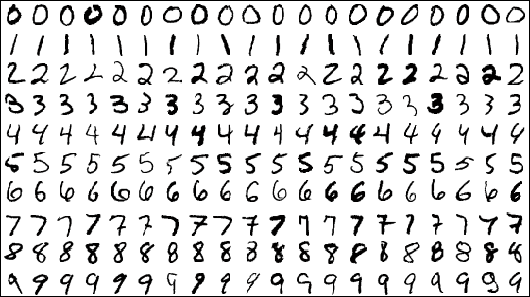
\includegraphics[width=2.4in]{mnist.png}
      \end{center}
    \end{frame}
    
\begin{frame}{Experiment parameters}
  \begin{itemize}
       \item{ \textbf{Network structures} }
     \begin{itemize}
			\item{\# Layers : }
			\item{\# Nodes : }
			\item{\# Bias : }
			\item{What else?}       
     \end{itemize}
     \item{ \textbf{Activation function}}
     \begin{itemize}
      		\item{Sigmoid function}
      		\begin{align*}
      		& \sigma(z)=\frac{1}{1+e^{-z}}\\
      		& \sigma'(z)=\sigma(z)(1-\sigma(z))
      		\end{align*}
%      		\item{Mean Square Error}
%      		\begin{align*}
%      		& \mathcal{L}^k_{MSE}(\theta)=\frac{1}{M}\sum_{i=s_k}^{s_k+M}(y_i-f(x_i;\theta))^2
%      		\end{align*}
    \end{itemize}
    \item{ \textbf{Hyperparameters} }
    \begin{itemize}
    	\item {Learning rate $\alpha$ : }
    	\item {Regularization : None }
    	\item {\# Epochs : 50? }
    	\item {Size of Mini Batch : 1000? }
    	\item {What else?}
    \end{itemize}
  \end{itemize}
\end{frame}


\begin{frame}{Parallel experiments}
	\begin{itemize}
	\item { \textbf{PThreads} }
		\begin{itemize}
		\item {About PThreads setting}
		\end{itemize}
	\item { \textbf{CUDA} }
		\begin{itemize}
		\item {About CUDA setting}
		\end{itemize}
	\item { \textbf{theano} }
		\begin{itemize}
		\item {About theano}
		\end{itemize}
	\end{itemize}

\end{frame}